% This file was created with tikzplotlib v0.10.1.
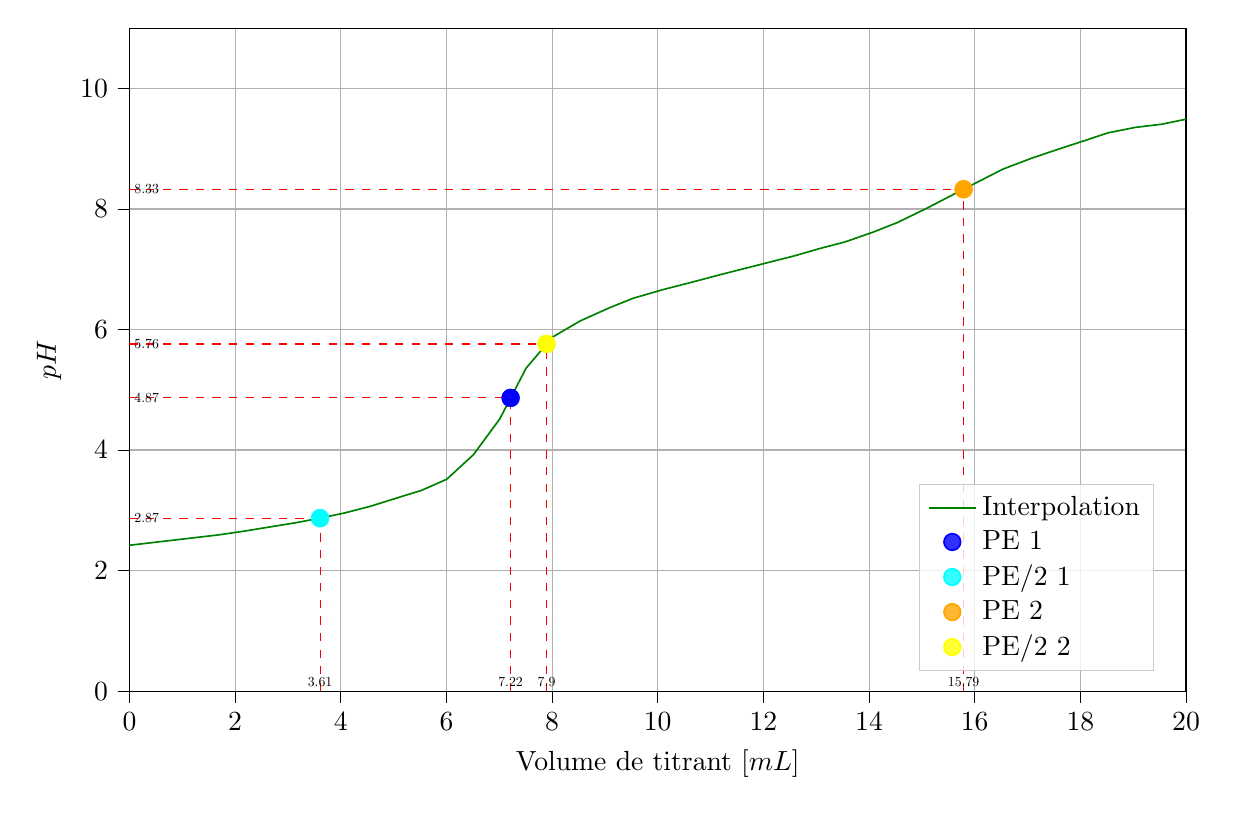
\begin{tikzpicture}

\definecolor{cyan}{RGB}{0,255,255}
\definecolor{darkgray176}{RGB}{176,176,176}
\definecolor{green}{RGB}{0,128,0}
\definecolor{lightgray204}{RGB}{204,204,204}
\definecolor{orange}{RGB}{255,165,0}
\definecolor{yellow}{RGB}{255,255,0}

\begin{axis}[
height=10cm,
legend cell align={left},
legend style={
  fill opacity=0.8,
  draw opacity=1,
  text opacity=1,
  at={(0.97,0.03)},
  anchor=south east,
  draw=lightgray204
},
tick align=outside,
tick pos=left,
width=15cm,
x grid style={darkgray176},
xlabel={Volume de titrant \(\displaystyle [mL]\)},
xmajorgrids,
xmin=0, xmax=20,
xtick style={color=black},
y grid style={darkgray176},
ylabel={$pH$},
ymajorgrids,
ymin=0, ymax=11,
ytick style={color=black}
]
\draw [red,dashed] (axis cs:0,4.87) -- (axis cs:7.22,4.87);
\draw [red,dashed] (axis cs:7.22,0) -- (axis cs:7.22,4.87);
\draw [red,dashed] (axis cs:0,2.87) -- (axis cs:3.61,2.87);
\draw [red,dashed] (axis cs:3.61,0) -- (axis cs:3.61,2.87);
\draw [red,dashed] (axis cs:0,8.33) -- (axis cs:15.79,8.33);
\draw [red,dashed] (axis cs:15.79,0) -- (axis cs:15.79,8.33);
\draw [red,dashed] (axis cs:0,5.76) -- (axis cs:7.9,5.76);
\draw [red,dashed] (axis cs:7.9,0) -- (axis cs:7.9,5.76);
\addplot [semithick, green]
table {%
0 2.42000007629395
1.66299998760223 2.58956003189087
2.16700005531311 2.65337991714478
3.16799998283386 2.79688000679016
3.66799998283386 2.88023996353149
4.08400011062622 2.95847988128662
4.55700016021729 3.06595993041992
5.1710000038147 3.23446011543274
5.52799987792969 3.33064007759094
6.00799989700317 3.51640009880066
6.51100015640259 3.92298007011414
7.01000022888184 4.51700019836426
7.50899982452393 5.3593602180481
8.00899982452393 5.87468004226685
8.5310001373291 6.14239978790283
9.08800029754639 6.36168003082275
9.53499984741211 6.51910018920898
10.085000038147 6.65869998931885
10.6719999313354 6.79127979278564
11.1680002212524 6.90696001052856
12.5830001831055 7.22158002853394
13.085000038147 7.34870004653931
13.5419998168945 7.45260000228882
14.0869998931885 7.61957979202271
14.543999671936 7.778480052948
15.08899974823 8.0109395980835
15.6809997558594 8.27964019775391
16.1770000457764 8.50142002105713
16.5300006866455 8.66020011901855
17.0869998931885 8.84609985351562
17.6749992370605 9.01900005340576
18.1669998168945 9.16009998321533
18.5289993286133 9.26521968841553
19.0419998168945 9.35420036315918
19.5410003662109 9.40738010406494
20 9.48999977111816
};
\addlegendentry{Interpolation}
\addplot [semithick, blue, mark=*, mark size=3, mark options={solid}, only marks]
table {%
7.21500015258789 4.86549997329712
7.21500015258789 4.86549997329712
};
\addlegendentry{PE 1}
\addplot [semithick, cyan, mark=*, mark size=3, mark options={solid}, only marks]
table {%
3.60800004005432 2.86944007873535
3.60800004005432 2.86944007873535
};
\addlegendentry{PE/2 1}
\addplot [semithick, orange, mark=*, mark size=3, mark options={solid}, only marks]
table {%
15.789999961853 8.32759952545166
15.789999961853 8.32759952545166
};
\addlegendentry{PE 2}
\addplot [semithick, yellow, mark=*, mark size=3, mark options={solid}, only marks]
table {%
7.89599990844727 5.76183986663818
7.89599990844727 5.76183986663818
};
\addlegendentry{PE/2 2}
\draw (axis cs:7.215,0) node[
  scale=0.5,
  anchor=south,
  text=black,
  rotate=0.0
]{7.22};
\draw (axis cs:0,4.8655) node[
  scale=0.5,
  anchor=west,
  text=black,
  rotate=0.0
]{4.87};
\draw (axis cs:3.608,0) node[
  scale=0.5,
  anchor=south,
  text=black,
  rotate=0.0
]{3.61};
\draw (axis cs:0,2.86944) node[
  scale=0.5,
  anchor=west,
  text=black,
  rotate=0.0
]{2.87};
\draw (axis cs:15.79,0) node[
  scale=0.5,
  anchor=south,
  text=black,
  rotate=0.0
]{15.79};
\draw (axis cs:0,8.3276) node[
  scale=0.5,
  anchor=west,
  text=black,
  rotate=0.0
]{8.33};
\draw (axis cs:7.896,0) node[
  scale=0.5,
  anchor=south,
  text=black,
  rotate=0.0
]{7.9};
\draw (axis cs:0,5.76184) node[
  scale=0.5,
  anchor=west,
  text=black,
  rotate=0.0
]{5.76};
\end{axis}

\end{tikzpicture}
